
\documentclass[12pt]{report}
\usepackage[french]{babel}
\usepackage[utf8]{inputenc}
\usepackage{csquotes}
\usepackage[T1]{fontenc}
\usepackage{eurosym}
\usepackage{ulem}
\usepackage[a4paper,left=2.5cm,right=2.5cm,top=2.5cm,bottom=3cm]{geometry}
%\usepackage{libertine}
\usepackage{graphicx}
\usepackage{enumitem}
\usepackage{wrapfig}
\usepackage{tikz}
\usepackage{lscape}
\usepackage{multicol}
\usepackage{hyperref}
\usepackage[toc]{appendix}
\hypersetup{
    colorlinks=true,
    linkcolor=black,
    filecolor=magenta,
    urlcolor=blue,
}
\urlstyle{same}

\usepackage{tabto}

\usepackage{siunitx}
\usepackage{caption}
\usepackage{subcaption}

\usepackage[]{biblatex}
\addbibresource{sample.bib}

\setlength{\parindent}{0cm}
\setlength{\parskip}{1ex plus 0.5ex minus 0.2ex}
\newcommand{\hsp}{\hspace{20pt}}
\newcommand{\HRule}{\rule{\linewidth}{0.5mm}}

\begin{document}

\begin{titlepage}
    \begin{sffamily}
    \begin{center}
    \Huge Can You Catch It ?
    \normalsize \\ IDASM104: Projet interdisciplinaire \\[0.5cm]

    
\includegraphics[height=9cm]{images/unamur.png}
    \\[2cm]

    
    ALBRECQ Jean, PETIT Antoine, \\ LAMBART Cyprien, DEGUELDRE Jessica
    \\[0.5cm]

    \vfill

    % Bottom of the page
    {\large Professeurs: S. Faulkner B. Frénay V. Salnikov. \\ 2020-2021}
    
    \end{center}
    \end{sffamily}
\end{titlepage}
\newpage

\tableofcontents
\newpage

\chapter{Introduction}
Le but de ce rapport est d'expliquer la démarche et la méthodologie qui a guidé l'élaboration des modèles et de l'analyse des données fournie par les \textit{opendata stib-mivb}. Ce rapport est constitué des différentes parties: l'analyse et la préparation des données, l'entraînement des modèles de régression et de classification et l'analyse de leurs résultats.

L'étape d'analyse et la préparation des données met en lumière les notions de normalisation, la détecteur d'\textit{outliers}, la selection de \textit{features}. La visualisation des données est également une partie importante de l'analyse des données. En suite dans l'étape d'entraînement des modèles passe par un phase de selection des méta-paramètres et d'optimisation des prédictions.

\section{Présentation du projet}
Il nous a été demandé de développer un nouveau service ou une analyse pertinente par rapport au défis de la mobilité. Plusieurs opendata nous était proposées, nous avons décidé de choisir celle de la STIB. Nous avons choisi de mettre en place un service permettant de savoir si prochain bus qui arrivera à un stop que l'on attend aura du retard ou non.

\chapter{Préparation et visualisation des données}

\section{Récolte des données}
La première étape est de toute évidence la récolte des données. Notre projet nous demandais d'avoir accès à un historique de retard mais malheureusement cette historique ne fait pas partie des datasets des opendata STIB. Nous avons donc développé un script python\footnote{Le code de ce script est disponible à l'adresse suivante: \href{https://github.com/jalbrecq/CanYouCatchIt/blob/main/sandbox/delay_gathering/delay_gathering.py}{lien github du script}} nous permettant de constituer cet historique de retard. Pour obtenir le délais, le script compare le temps d'arrivée théorique (qui nous est fournis par les fichiers GTFS\footnote{General Transit Feed Specification}) et l'heure d'arrivée prévue (qui nous est fournie par l'api "\textit{waiting time}"). Le délais est enregistré dans un fichier csv. En plus du délais, le script enregistre la température, la vitesse du vent, l'humidité et la visibilité grâce à l'api OpenWeather\footnote{Documentation disponible \href{https://openweathermap.org/}{ici}}. Un nouveau fichier csv est généré chaque jour.

Nous avons dans un premier temps récolté les données pour deux stop (les numéros 0089 et 6608G, voir leur emplacement dans l'annexe \ref{appendix:stop_pos_1}) du premier novembre au douze novembre. Les fichiers csv sont disponibles sur le \textit{repository}\footnote{Disponible \href{https://github.com/jalbrecq/CanYouCatchIt/tree/main/sandbox/data/csv}{ici}} du projet. Dans un second temps, nous avons récolté les données de tout les stops d'une ligne de bus (la ligne 39). La position de tout les stops de la ligne sont visible sur l'annexe \ref{appendix:stop_pos_2}\footnote{Une carte GoogleMyMaps est également disponible \href{https://www.google.com/maps/d/edit?mid=1_qNGPUfuZXrqC3UZXkmDOWuhEHJfYAox&usp=sharing}{ici}}. Les données récoltées durant cette deuxième phase sont disponible sur le \textit{repository} du projet\footnote{Disponible \href{https://github.com/jalbrecq/CanYouCatchIt/tree/main/sandbox/data/csv2}{ici}}.

\section{Préparation des données}

\subsection{Normalisation}
Une fois les données recueillies, nous avons vérifié si elle devaient être normalisés ou non. Après une rapide analyse du dataset généré par le script, il nous a semblé évidant qu'une phase de normalisation était indispensable.

\subsection{Suppression des outliers}


\begin{appendices}
    \chapter{Position des stops}
    \begin{figure}
        \centering
        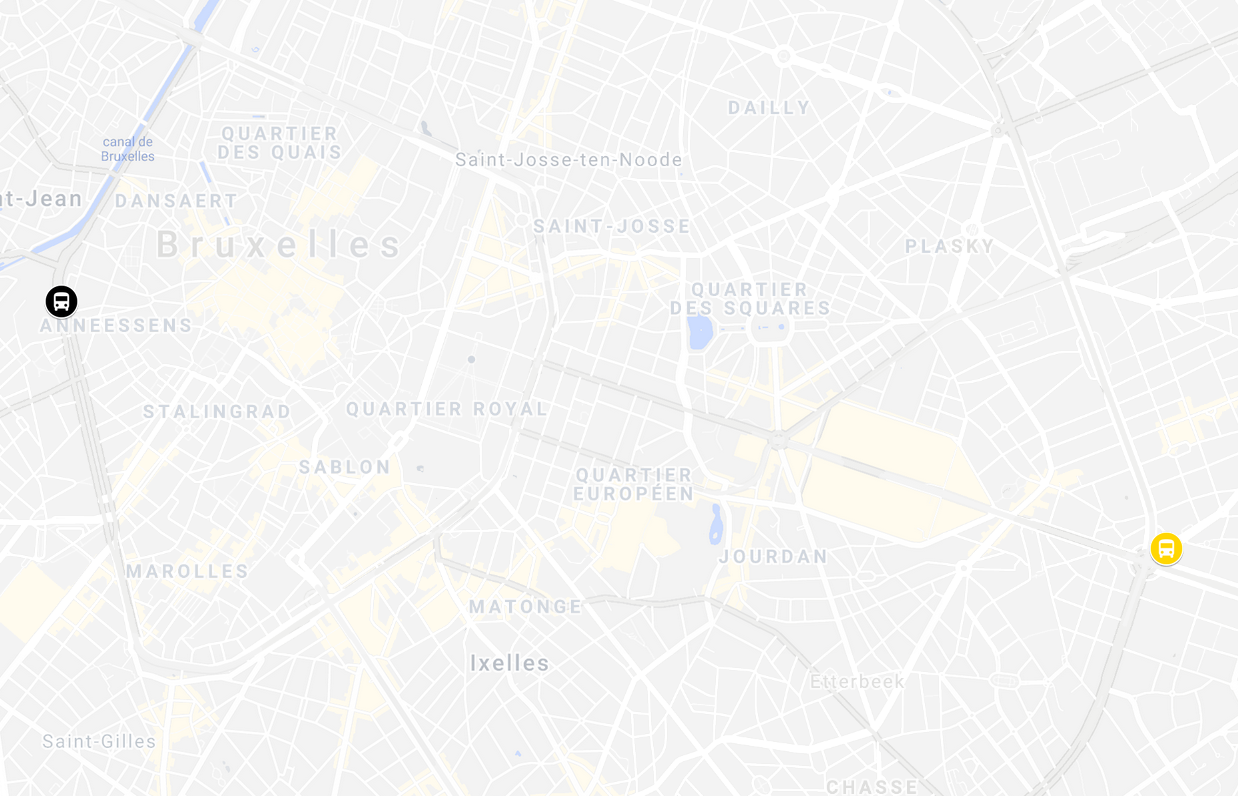
\includegraphics[width=0.9\textwidth]{images/stop_pos_1.png}
        \caption{Position des stops numéro 0089 et 6608G en jaune et noir respectivement.}
        \label{appendix:stop_pos_1}
    \end{figure}

    \begin{figure}
        \centering
        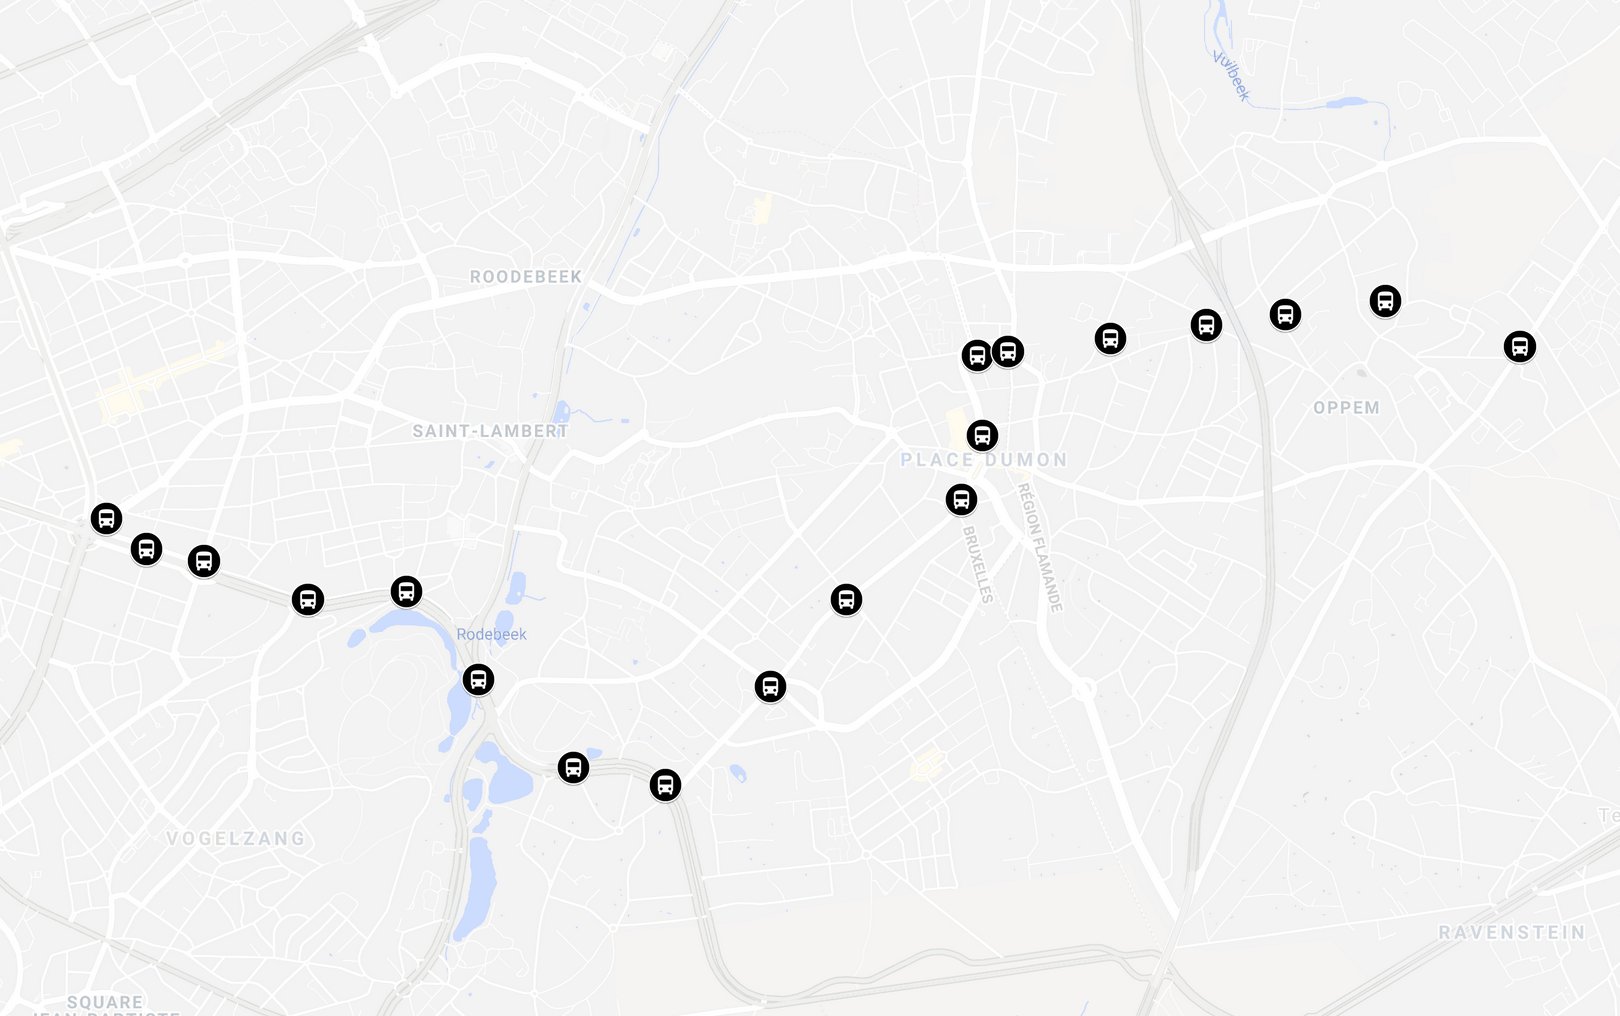
\includegraphics[width=0.9\textwidth]{images/stop_pos_2.png}
        \caption{Position des stops présent sur la ligne 39}
        \label{appendix:stop_pos_2}
    \end{figure}

\end{appendices}

\nocite{*}
\printbibliography
\end{document}
